\begin{figure*}[t]
\vskip 0.2in
\begin{center}


\includegraphics[width=0.8\columnwidth]{figures/pca_legend.pdf}

\subfigure{
{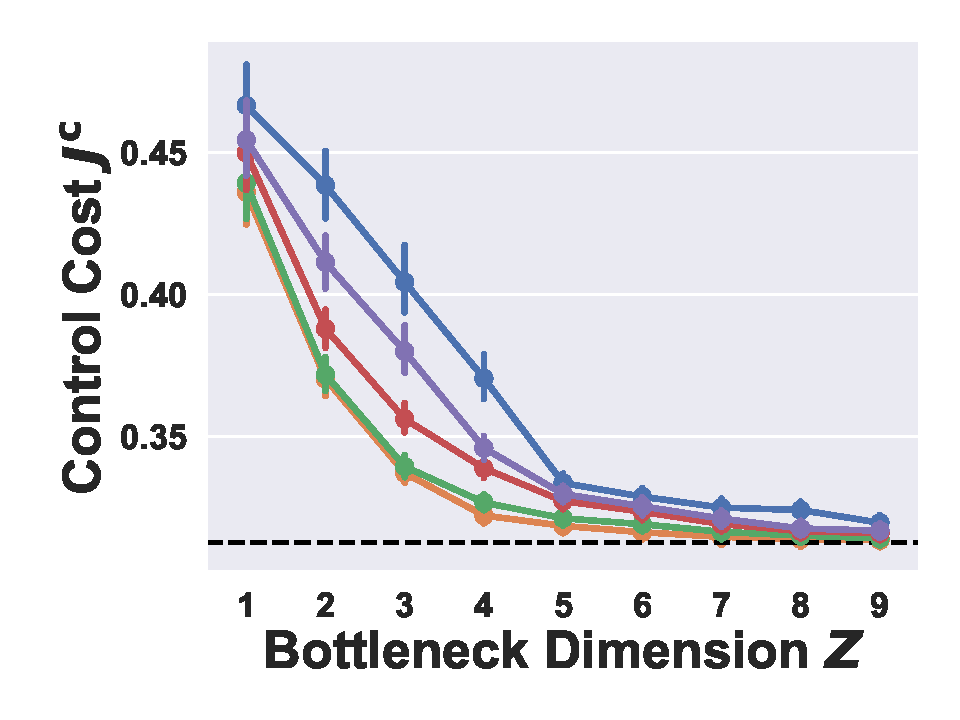
\includegraphics[width=0.4\columnwidth]{figures/pca_full/pca_full_cost_bottleneck.pdf}}
\label{fig_pca_full_cost_bottleneck}
}
\subfigure{
{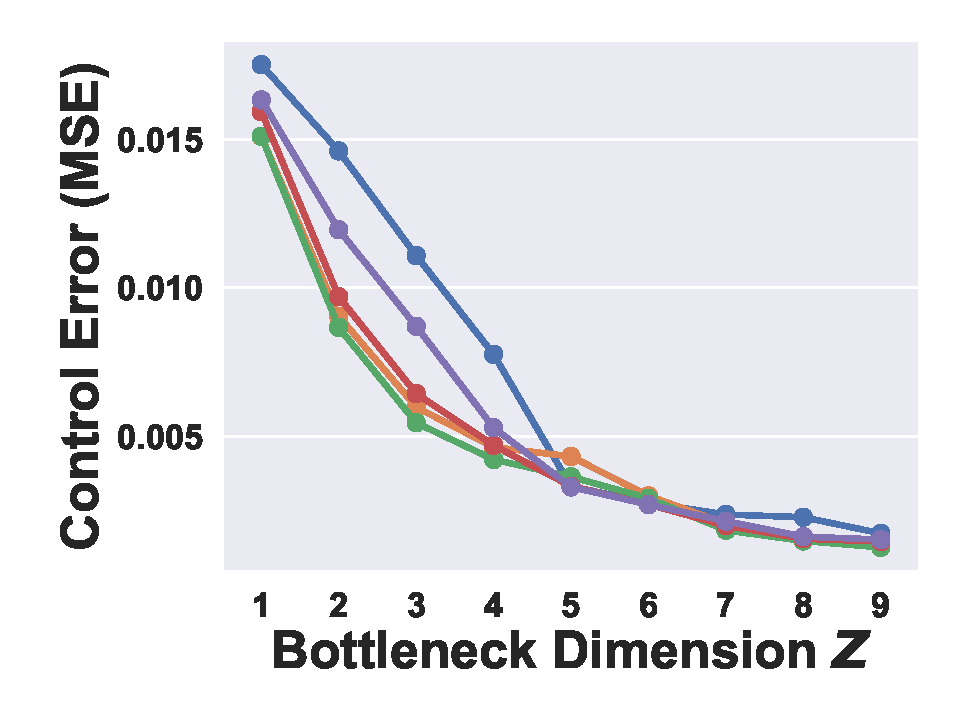
\includegraphics[width=0.4\columnwidth]{figures/pca_full/pca_full_ctrl_MSE.pdf}}
\label{fig_pca_full_ctrl_MSE}
}
\subfigure{
{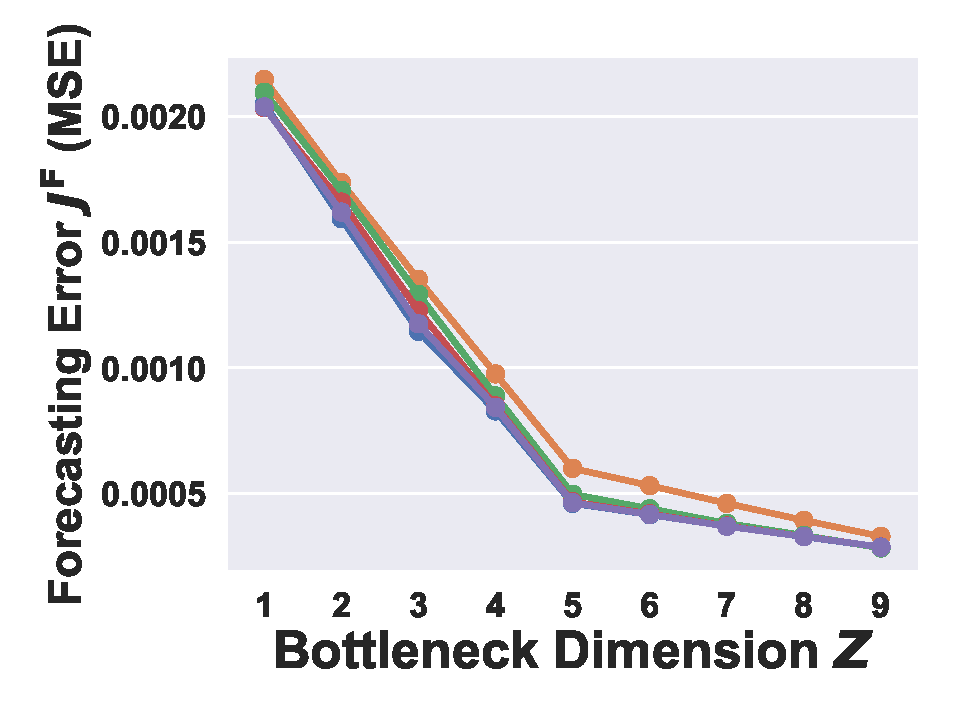
\includegraphics[width=0.4\columnwidth]{figures/pca_full/pca_full_fcst_MSE.pdf}}
\label{fig_pca_full_fcst_MSE}
}
\subfigure{
{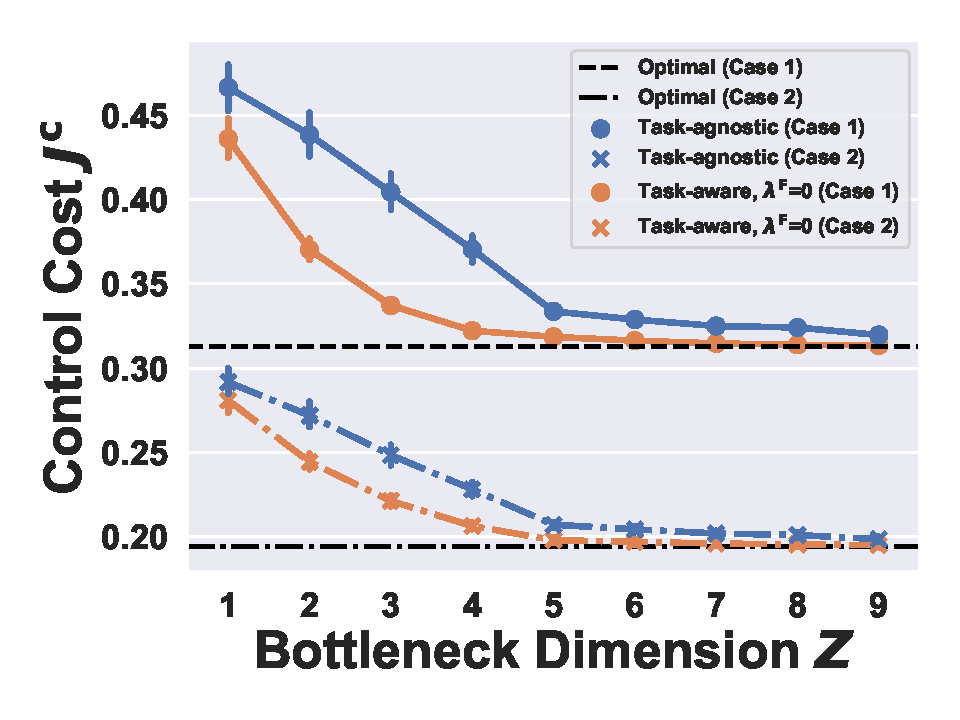
\includegraphics[width=0.4\columnwidth]{figures/pca_full/pca_cost_bottleneck_combined.pdf}
\label{fig_pca_full_forecast_errors}
}
}
\caption{\textbf{Analytic results for linear control:} (a) By only representing information salient to a control task, our co-design method (orange) achieves the optimal control cost with  
$43\%$
% $1.75\times$ 
less data than a standard MSE approach (``task-agnostic'', blue). Formal definitions of all benchmarks are in Sec. \ref{sec:evaluation}. (b-c) By weighting prediction error by $\lambdaforecast > 0$, we learn representations that are compressible, have good predictive power, and lead to near-optimal control cost (\eg~ $\lambdaforecast=1.0$).
(d) For the \textit{same} timeseries $\bolds$, two different control tasks require various amounts of data shared, motivating our task-centric representations.}
% \caption{\textbf{Analytic Results for Linear Control:} (a) By compressing information salient to a control task, our co-design method (orange) can effectively lower the control cost than a standard RMSE approach (``task-agnostic'', blue). Formal definitions of all benchmarks are in Sec. \ref{sec:evaluation}. (b-c) By weighting prediction error by $\lambdaforecast > 0$, we learn representations that are compressible, have good predictive power, and lead to near-optimal control cost (\eg $\lambdaforecast=1.0$).
% (d) For the \textit{same} timeseries $\bolds$ but a different control task (bottom), co-design method may not differ too much from the standard RMSE approach.}
\label{fig:main_pca_full}
\end{center}
\vskip -0.2in
\end{figure*}
